\section{Implementation Details for Linear Regression}\label{sec:linreg}

\textbf{Objective Function.} 
In this experiment, we define the objective function as $f(w) = \frac{1}{n}\sum_{i=1}^n (w^Tx_i - y_i)^2$ and $\tilde{f}(w) = (w^Tx_i - y_i)^2$ for a randomly sampled $i$.


\textbf{Synthetic Dataset.}
The data points $x_i$ were generated by $x_i \sim \mathcal{N}(0, \sigma_x^2I)$. 
We then chose target weights $w_{\text{init}}$ uniformly at random in the range $[-1, 1]$, and generated the labels by $y_i \sim \mathcal{N}(w_{init}^T x_i, \sigma_u^2)$.
To generate the synthetic dataset, we set $d = 256$ and $\sigma_u = \sigma_x = 1$ and sampled $4096$ data points.

\begin{figure*}[t]
    \centering
    \subfigure[Log-log plot of linear regression]{
        \centering
        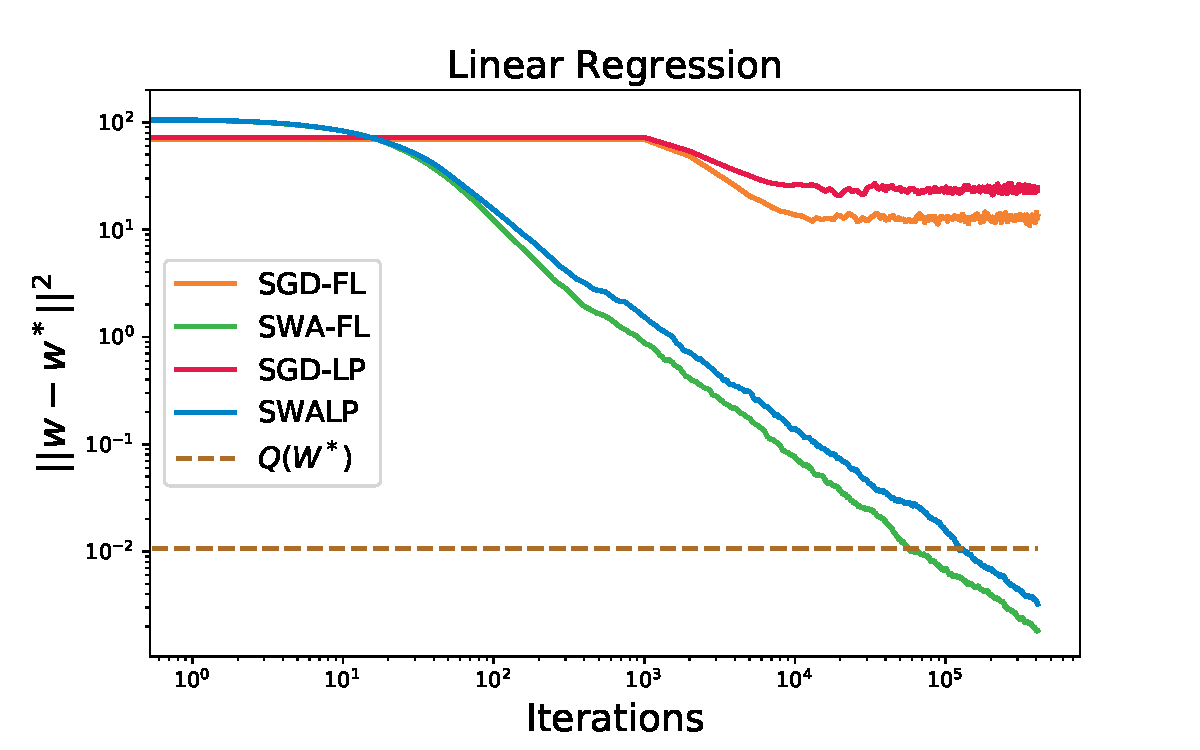
\includegraphics[width=0.4\textwidth]{figures/regression-log-log.pdf}\label{fig:log-log}
    }
    \subfigure[MNIST test error (\%) for logistic regression experiments. We varied the precisions used to train SGD-LP and SWALP.]{
        \centering
        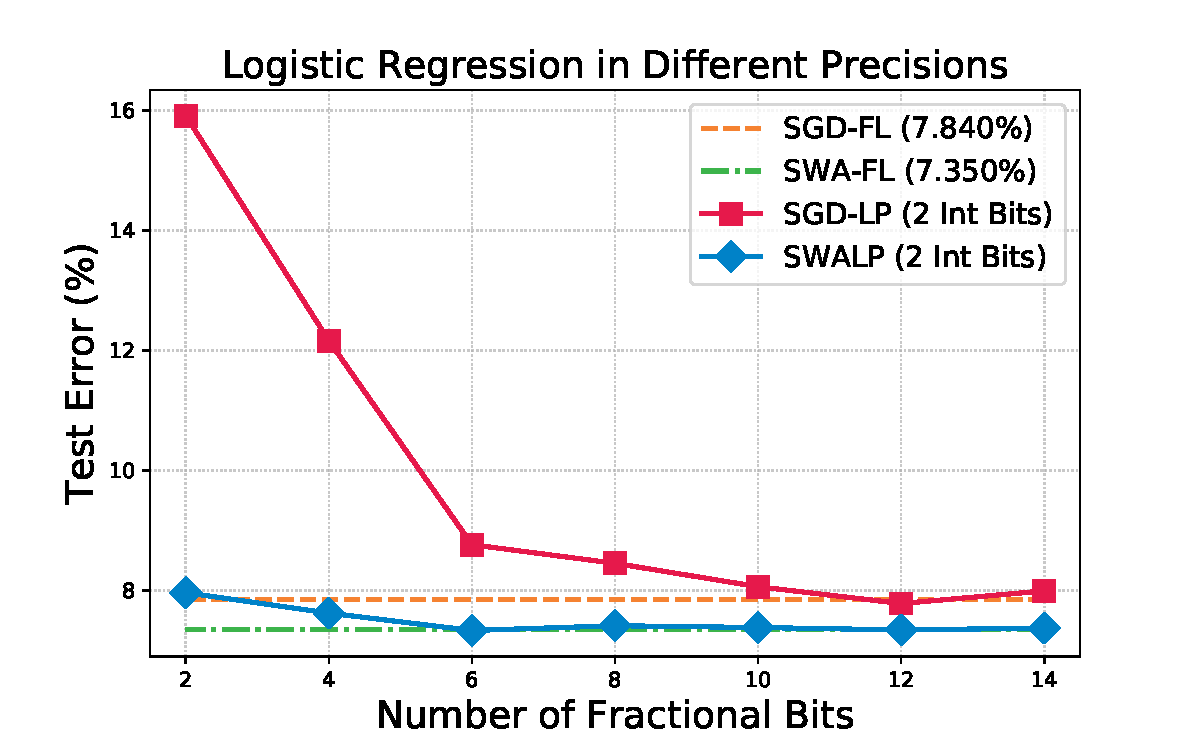
\includegraphics[width=0.45\textwidth]{figures/LogReg-Test-DiffBits.pdf}\label{fig:logreg-diff-prec-test}
    }
    \caption{More experimental results for linear and logistic regression.}
\end{figure*}


\textbf{Convergence.}
We plot the square distance between $w_t$ (or $\bar w_t$ for SWALP) and the optimal solution $w^*$ in log-log scale in Figure~\ref{fig:log-log}.
For reference, we also plot the squared distance between $Q(w^*)$ and $w^*$ to illustrate the size of quantization noise. It can be seen more clearly that the convergence rate is about $O(1/T)$.

\section{Implementation Details for Logistic Regression}\label{sec:logreg}

We use logistic regression with L2 regularization on MNIST dataset ~\cite{MNIST} .
In this experiment, we use the MNIST dataset~\cite{MNIST}. 
The objective function is defined as
$
    f(w) = - \frac{1}{n}\sum_{i=1}^n \log{(\operatorname{softmax}(w^Tx_i + b))} + \frac{\lambda}{2} \|w\|^2
$.
We choose $\lambda=10^{-4}$, a regularization parameter used in prior work~\cite{HALP,SVRG}, which makes the objective a strongly convex function with $M\ne 0$.
We use a learning rate of $\alpha = 0.01$ and cycle length $C=1$ for all four settings.
For this experiment we measure the norm of gradient at each iteration to illustrate the convergence of the algorithm; this is a more useful metric because MNIST is sparse and poorly conditioned, and it is a metric that has been used for logistic regression on MNIST in previous work~\cite{HALP}.
We warm up for 60000 iterations. 
For SWALP and SGD-LP, we use 4-bit word length and 2-bit fractional length.
For the experiment where we evaluate different precision, we use the same hyper-parameters, except the following: 1) the warm-up period is set to 600k iterations (i.e. 10 epochs); and 2) we report the final evaluation results after training for 3 million steps (i.e. 50 epochs). The test results is reported in Figure~\ref{fig:logreg-diff-prec-test}. As we could see the same conclusion still holds. Detail statistics is reported in Table~\ref{table:logreg-diffprec-stats}.

\begin{table}[H]
\centering
\caption{MNIST training and testing error (\%) for logistic regression experiment with different fractional bits for training.} 
\begin{tabular}{lccccc}

\toprule
 & & \multicolumn{2}{c}{SGD} & \multicolumn{2}{c}{SWA} \\
Format & Precision & Train Err   & Test Err  & Train Err   & Test Err  \\
\midrule
Float & 32 & 7.07 & 7.84 & 6.6 & 7.35 \\
\multirow{7}{*}{Fixed Point} & FL=14, WL=16 & 7.30 & 7.99 & 6.59 & 7.37 \\
 & FL=12, WL=14 & 7.18 & 7.78 & 6.59 & 7.34 \\
 & FL=10, WL=12 & 7.21 & 8.06 & 6.57 & 7.38 \\
 & FL=8, WL=10 & 7.82 & 8.45 & 6.61 & 7.41 \\
 & FL=6, WL=8 & 8.31 & 8.76 & 6.78 & 7.33 \\
 & FL=4, WL=6 & 11.64 & 12.16 & 7.21 & 7.62 \\
 & FL=2, WL=4 & 16.27 & 15.91 & 7.98 & 7.96 \\
\bottomrule
\end{tabular}
\label{table:logreg-diffprec-stats}
\end{table}

\section{Implementation Details for Section~\ref{sec:expr}}\label{sec:dlexp}
For VGG-16 and Pre-activation ResNet-164, we replicate the full precision baselines by using the publicly released implementation of SWA~\cite{SWA-repo}. Based on validation error, we discover that for low-precision training it is beneficial to decay the learning rate lower before SWA starts. Therefore, we follow the SGD learning rate schedule described in \citet{SWA} before SWALP starts. For ResNet-18 on ImageNet dataset, we follow the learning rate schedule described in \citet{resnet}.

We now disclose the specific hyperparameters.
\begin{itemize}
    \item For VGG-16 reported in \citet{SWA}, we use He's initialization \cite{he-init} and weight decay of \texttt{5e-4}. One budget is set to be $200$ epochs. For SGD-LP, we set the initial learning rate $\alpha_1=0.05$ for the first $0.5$ budget, and linearly decreased to $0.01 \alpha_1$ for $0.5-0.9$ budget, and keep the learning rate constant for $0.9-1.0$ budget. For SWALP, we use the same learning rate for the first $200$ epochs. We starts SWALP averaging at $200$th epoch and keep a constant learning rate $0.01$ with averaging frequency $c=1$ epoch. 
    \item For Preactivation ResNet-164, we use He's initialization \cite{he-init} and weight decay of \texttt{3e-4}. One budget is set to be $150$ epochs. For SGD, we use cycle length $C=1$ and set the initial learning rate $\alpha_1=0.1$ for the first $0.5$ budget, and linearly decreased to $0.01 \alpha_1$ for $0.5-0.9$ budget, and keep the learning rate constant for $0.9-1.0$ budget. For SWALP, we start averaging at $150$ epoch and keep a constant learning rate $0.01$ with averaging frequency $c=1$ epoch. Moreover, we found that possibly because low-precision training is less stable, it is better to average for less epochs. Therefore, we evaluate the full precision averaged model on a subset of the training set and report the performance of the model with lowest loss on this subset. 
    \item For ResNet-18 on ImageNet, we use weight decay \texttt{1e-4}. One budget is set to be 90 epochs. For both SGD and SGD-LP, we use initial learning rate $0.1$ and decay it by a factor of 10 every 30 epochs. For SWA and SWALP, we start averaging after 90 epochs with a constant learning rate of $0.001$ for SWA and $0.001$ for SWALP (obtained by a grid search). The averaging frequency is $c=1$ epochs. 
\end{itemize}
    
\clearpage
\section{Data for Figure~\ref{fig:diffc_qswa}}\label{sec:data-figure3}



\begin{table*}[h]
\label{table:figure3-data-diffc}

\caption{CIFAR100 classification error (\%) on test set. We use the same base model and average it with different frequency. Each column show how the SWA model perform on the test set during the training according to each averaging schedule. }
\centering
\begin{tabular}{@{}lllllllllllllll@{}}
\toprule
Epoch   & \multicolumn{2}{c}{1} & \multicolumn{2}{c}{5} & \multicolumn{2}{c}{10} & \multicolumn{2}{c}{50} & \multicolumn{2}{c}{80} & \multicolumn{2}{c}{90} & \multicolumn{2}{c}{100} \\
\#batch/avg & Error         & STD        & Error         & STD        & Error          & STD        & Error          & STD        & Error          & STD        & Error          & STD        & Error          & STD         \\ \midrule
1                 & 28.95       & 0.12       & 28.38       & 0.12       & 28.01        & 0.10       & 27.20        & 0.34       & 27.21        & 0.13       & 27.19        & 0.13       & 27.11        & 0.29        \\
2                 & 28.96       & 0.12       & 28.37       & 0.13       & 28.01        & 0.10       & 27.20        & 0.34       & 27.21        & 0.13       & 27.19        & 0.13       & 27.12        & 0.29        \\
20                & 28.96       & 0.24       & 28.32       & 0.12       & 28.02        & 0.04       & 27.20        & 0.33       & 27.21        & 0.11       & 27.20        & 0.15       & 27.14        & 0.28        \\
100               & 29.20       & 0.21       & 28.47       & 0.09       & 28.23        & 0.18       & 27.24        & 0.29       & 27.18        & 0.23       & 27.17        & 0.17       & 27.18        & 0.22        \\
200               & 29.63       & 0.31       & 28.74       & 0.15       & 28.25        & 0.14       & 27.27        & 0.29       & 27.23        & 0.21       & 27.17        & 0.14       & 27.20        & 0.20        \\
once/epoch                & 30.00       & 0.12       & 28.88       & 0.13       & 28.28        & 0.10       & 27.23        & 0.31       & 27.14        & 0.16       & 27.19        & 0.15       & 27.16        & 0.26        \\ \bottomrule
\end{tabular}
\end{table*}

\begin{table*}[h]
\label{table:figure3-data-qswa}
\caption{CIFAR100 classification error (\%) on test set. We use block floating point to quantize the average. Each column shows the result of using different number bits for the block floating point. }
\centering
\begin{tabular}{cccccccccc}
\toprule
\# of bits & Float            & 16               & 14               & 12               & 10               \\
Test Error & 26.65$\pm{0.29}$ & 26.65$\pm{0.29}$ & 26.66$\pm{0.29}$ & 26.65$\pm{0.29}$ & 26.60$\pm{0.33}$ \\
\midrule
\# of bits &  & 9                & 8                & 7                & 6 \\
Test Error &  & 26.67$\pm{0.28}$ & 26.85$\pm{0.38}$ & 27.48$\pm{0.38}$ & 29.48$\pm{0.25}$  \\
\bottomrule
\end{tabular}
\end{table*}
